\documentclass{article}
\usepackage[T1]{fontenc}
\usepackage{lmodern}
\usepackage{graphicx}
\usepackage{amsmath,amssymb}
\usepackage[a4paper,margin=2cm]{geometry}
\usepackage[absolute,overlay]{textpos}
\setlength{\TPHorizModule}{1mm}
\setlength{\TPVertModule}{1mm}
\usepackage[indonesian]{babel}
\usepackage{hyperref}
\setlength{\emergencystretch}{2em}
% unit: Halaman 38

\begin{document}

% === Halaman 38 (llm) ===

\vspace{225.72mm}

Run program

% deskripsi: Screenshot kode program Python untuk enkripsi dan dekripsi menggunakan transposition cipher beserta output eksekusinya.
% bbox normalisasi: [0.0900, 0.1300, 0.8600, 0.8900]
\begin{textblock*}{161.70mm}(18.90mm,38.61mm)
\noindent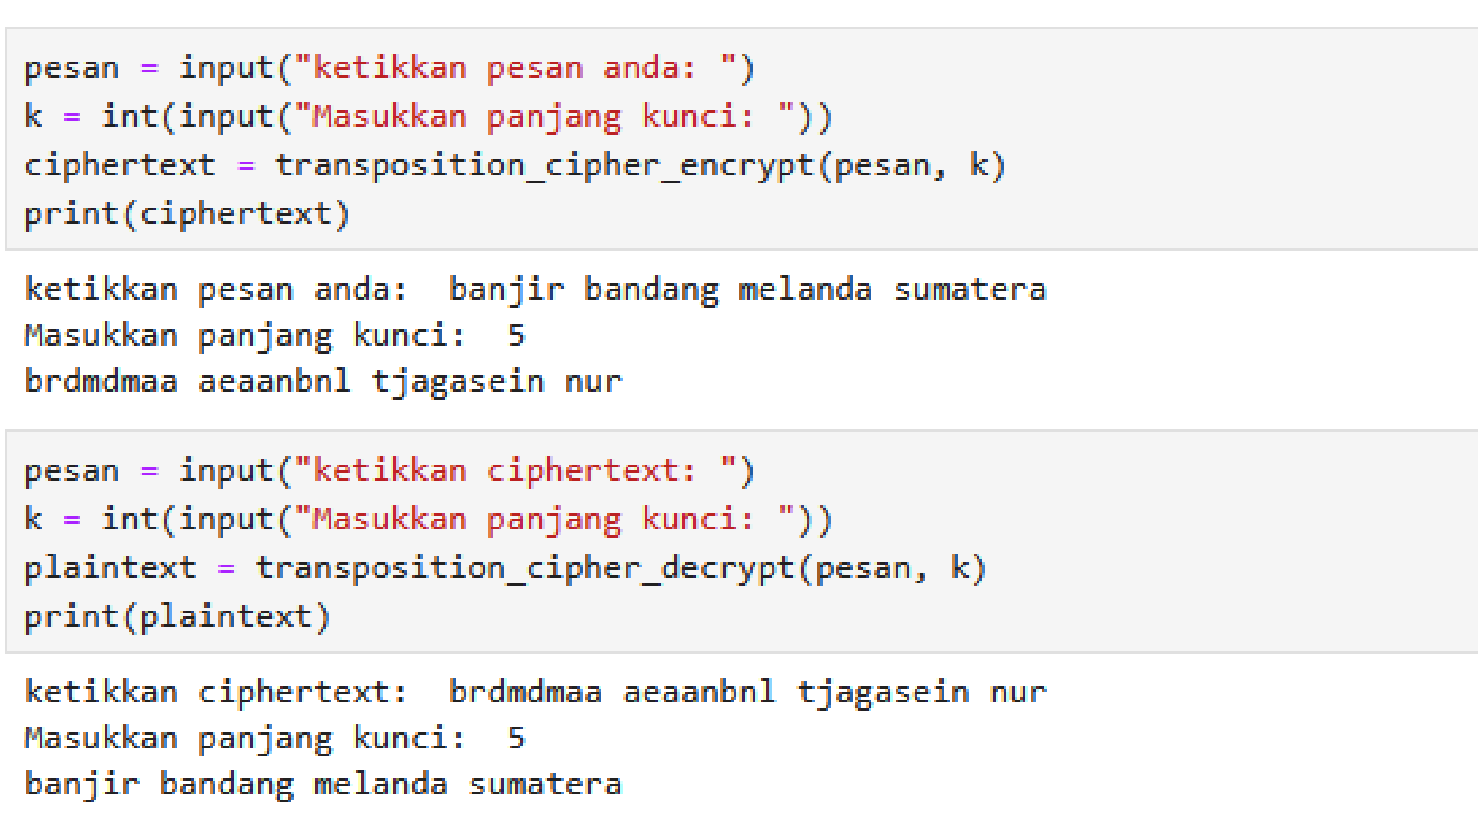
\includegraphics[width=161.70mm,height=225.72mm]{../../images/llm/page_038_img_01.png}%
\end{textblock*}

\end{document}
